\documentclass{beamer}

\mode<presentation>
{
  \usetheme{Frankfurt}
  \usecolortheme{orchid}
  \setbeamercovered{invisible}
  \setbeamertemplate{footline}[frame number]
}

\usepackage[english]{babel}
\usepackage[latin1]{inputenc}
\usepackage{times}
\usepackage[T1]{fontenc}
\usepackage{tikz}
\usepackage{array}

\def\blue{\color{blue}~}
\def\black{\color{black}~}


\usepackage{remreset}
\makeatletter
\@removefromreset{subsection}{section}
\makeatother
\setcounter{subsection}{1}

\title{Discrete Mathematics, Section 002, Spring 2016}
\subtitle{Lecture 3: Counterexamples,Boolean Algebra, Lists
}

\author[Zsolt]{Zsolt Pajor-Gyulai \\ \texttt{zsolt@cims.nyu.edu}}

\date{September 14, 2016}

\pgfdeclareimage[height=1cm]{NYUlogo}{NYUlogo.jpg}

\institute[NYU] 
{
\normalsize Courant Institute of Mathematical Sciences
}
\titlegraphic{\pgfuseimage{NYUlogo}}

\begin{document}

\begin{frame}
  \titlepage
\end{frame}

\AtBeginSection[]
{
\begin{frame}
\frametitle{Outline}
\tableofcontents[currentsection]
\end{frame}}

\begin{frame}{Refresher question}
\begin{block}{Question}
A logician just had a child. A friend of hers asks her if it's a boy or a girl. What is her answer?
\end{block}\pause
\begin{block}{Answer}
Yes.
\end{block}
\end{frame}

\section{Counterexamples}

\begin{frame}{How do we show if a statement is false?}
\begin{itemize}
\item Show that it implies a contradiction. $\qquad\rightarrow\qquad\textrm{Later}$\pause
\item Come up with a counterexample. $\qquad\rightarrow\qquad\textrm{Now}$.
\end{itemize}\pause
\vspace{0.4cm}
For example:
\begin{block}{False claim}
Let $a$ and $b$ be integers. If $a|b$ and $b|a$, then $a=b$.
\end{block}\pause

If I can find just one pair $a$, $b$ that are not equal but they divide each other, then I can refute the statement!\pause
\[
a=5, b=-5\qquad\rightarrow\qquad 5\cdot (-1)=-5,\qquad (-5)\cdot (-1) = 5
\]
This works!
\end{frame}

\begin{frame}{How do we show if a statement is false?}
\begin{block}{Refuting a false if-then statement via a counterexample.}
To disprove a statement of the form 'If $A$, then $B$': Find an instance where $A$ is true but $B$ is false.
\end{block}\pause

\begin{itemize}
\item Easier than proving true statements in general.\pause
\item Finding counterexamples can be tricky!\pause
\item Try to create strange examples!
\end{itemize}

When you do not know whether a statement is true or false:
\begin{itemize}
\item Try proving it!\pause
\item When you get stuck, try to figure out what the problem is and whether it suggests that there should be a counterexample.
\end{itemize}
\end{frame}

\begin{frame}{Example}
\begin{block}{False claim}
Let $a$ and $b$ be integers. If $a|b$ and $b|a$, then $a=b$.
\end{block}

\begin{block}{Proof attempt}
Let $a$ and $b$ be integers with $a|b$ and $b|a$. \uncover<2->{\color{blue}Since $a|b$, there is an integer $x$ such that $b=ax$. Since $b|a$, there is an integer $y$ such that $a=by$.}~~\color{black}$\dots$ Therefore $a=b$.\qed
\end{block}

\uncover<3->{While trying to bridge the gap, it looks like we should show $x=y=1$.
\[
a=by\qquad\rightarrow\qquad a=(ax)y\qquad\rightarrow\qquad a=(xy)a
\]
}
\uncover<4->{Only shows that $xy=1$.$\qquad\rightarrow\qquad$ $x=y=-1$ works too!}

\uncover<5->{\center{\color{blue}This would yield $a=-b$ and now it is easy to pick the counterexample.\color{black}}}
\end{frame}


\section{Boolean Algebra}
\begin{frame}[t]{Ordinary Algebra}
Useful for reasoning about numbers:
\[
x^2-y^2=(x-y)(x+y)\qquad\textrm{Holds for any numbers $x$ and $y$}
\]\pause
\begin{itemize}
\item Letters stand for numbers.\pause
\item Operators are the usual ones: $+,-,\cdot,/$\pause
\item Value of an expression like $3x-4$ depends on $x$.\pause
\item When e.g. $x=1$, the value is $3(-1)-4=-1$.
\end{itemize}
\end{frame}

\begin{frame}[t]{Boolean Algebra}
Useful dealing with statements.
\begin{itemize}
\item Letters stand for the values \blue True\black or \blue False\black. (Two values!)\pause
\item Operators: and ($\wedge$), or ($\vee$), not ($\neg$), etc. \pause
\item We can create and evaluate more complicated \textbf{Boolean expressions}:
\[
\neg(x\wedge y)\qquad (\neg x)\vee (\neg y)
\]\pause
\item Values of expressions can be summarized in \textbf{Truth tables}.
\end{itemize}


\only<4>{\begin{figure}
Truth table of $x\wedge y$ (AND):
\centering
\[
\begin{tabular}{| >{\centering\arraybackslash}b{1in} | >{\centering\arraybackslash}b{1in} || >{\centering\arraybackslash}b{1in}|}
\hline
x& y &x$\wedge$ y\\
\hline
True & True & True\\
True & False& False\\
False & True & False\\
False & False & False\\
\hline
\end{tabular}
\]
\end{figure}}

\only<5>{\begin{figure}
Truth table of $x\vee y$ (OR):
\centering
\[
\begin{tabular}{| >{\centering\arraybackslash}b{1in} | >{\centering\arraybackslash}b{1in} || >{\centering\arraybackslash}b{1in}|}
\hline
x& y &x$\vee$ y\\
\hline
True & True & True\\
True & False& True\\
False & True & True\\
False & False & False\\
\hline
\end{tabular}
\]
\end{figure}}

\only<6>{\begin{figure}
Truth table of $\neg x$  (NOT):
\centering
\[
\begin{tabular}{| >{\centering\arraybackslash}b{1in}|| >{\centering\arraybackslash}b{1in}|}
\hline
x& $\neg$ x\\
\hline
True & False\\
False & True\\
\hline
\end{tabular}
\]
\end{figure}}

\end{frame}




\begin{frame}{Identities}
\begin{itemize}
\item In ordinary algebra, you cannot check
\[
(x+y)^2=x^2+2xy+y^2
\]
for (infinitely many) every number $x$ and $y$.\pause
\item However, look at\vspace{-0.2cm}
\[
\neg(x\wedge y)\qquad (\neg x)\vee (\neg y)
\]
\[
\begin{tabular}{| >{\centering\arraybackslash}b{0.2in} | >{\centering\arraybackslash}b{0.2in} || >{\centering\arraybackslash}b{0.3in}| >{\centering\arraybackslash}b{0.6in}|| >{\centering\arraybackslash}b{0.3in} |>{\centering\arraybackslash}b{0.3in}|>{\centering\arraybackslash}b{0.8in}|}
\hline
x& y &x$\wedge$ y& $\neg(x\wedge y)$& $\neg$ x& $\neg$ y & ($\neg$ x)$\vee$ ($\neg$ y)\\
\hline
T & T& T & F&F&F&F\\
T & F& F& T&F&T&T\\
F & T & F& T&T&F&T\\
F & F & F& T&T&T&T\\
\hline
\end{tabular}
\]
\end{itemize}
\pause
\center{We say $\neg(x\wedge y)$ and $(\neg x)\vee (\neg y)$ are \textbf{logically equivalent}.}
\end{frame}

\begin{frame}[t]
\begin{block}{Truth table proof of logical equivalence}
To show that two Boolean expressions are logically equivalent: Construct a truth table showing the values of the two expressions for all possible values of the variables.
\end{block}

\only<2>{
Basic algebraic properties of the operations $\wedge,\vee,\neg$:
\begin{itemize}
\item \textbf{(Commutative properties)} 
\[
x\wedge y=y\wedge x\qquad,  x\vee y=y\vee x.
\]
\item (\textbf{Associative properties})
\[
(x\wedge y)\wedge z = x\wedge (y \wedge z),\qquad (x\vee y)\vee z = x\vee (y\vee z). 
\]
\item (\textbf{Identity elements}) 
\[
x\wedge True=x,\qquad x\vee False=x.
\]
\end{itemize}}

\only<3>{
\begin{itemize}
\item \textbf{(Distributive properties)} 
\[
x\wedge (y\vee z)=(x\wedge y)\vee (x\wedge z), \qquad  x\vee (y\wedge z)=(x\vee y)\wedge(x\vee z).
\]
\item (\textbf{DeMorgan's Laws})
\[
\neg(x\wedge y)=(\neg x)\vee (\neg y),\qquad \neg(x\vee y)=(\neg x)\wedge(\neg y).
\]
\item $\neg(\neg x)=x$.
\item $x\wedge x=x$ and $x\vee x$.
\item $x\wedge(\neg x)=False$ and $x\vee(\neg x)=True$.
\end{itemize}}

\end{frame}

\begin{frame}{Further logical operators}
\begin{itemize}
\item The operations $\wedge$, $\vee$, $\neg$ were created to replicate mathematicians use of the words \emph{and}, \emph{or}, \emph{not}. \pause
\item We also introduce \emph{implies} ($\rightarrow$) and \emph{if-and-only-if} ($\leftrightarrow$).
\end{itemize}\pause
\vspace{-0.2cm}
\begin{figure}
\centering
\small{Models $A\Rightarrow B$, only false when $A$ is true but $B$ is not.}
\[
\begin{tabular}{| >{\centering\arraybackslash}b{1in} | >{\centering\arraybackslash}b{1in} || >{\centering\arraybackslash}b{1in}|}
\hline
x& y &x$\rightarrow$ y\\
\hline
True & True & True\\
True & False& False\\
False & True & True\\
False & False & True\\
\hline
\end{tabular}
\]
\small{Models $A\Leftrightarrow B$, false when one is true but the other one is false.}
\[
\begin{tabular}{| >{\centering\arraybackslash}b{1in} | >{\centering\arraybackslash}b{1in} || >{\centering\arraybackslash}b{1in}|}
\hline
x& y &x$\leftrightarrow$ y\\
\hline
True & True & True\\
True & False& False\\
False & True & False\\
False & False & True\\
\hline
\end{tabular}
\]
\end{figure}
\end{frame}

%\begin{frame}
%These can be expressed however in terms of the basic operators.
%\end{frame}

\section{Lists}

\begin{frame}{Collections}
In this course we consider two types of collections:
\begin{itemize}
\item \textbf{Lists}: Ordered collections.\pause
\item \textbf{Sets}: Unordered collections.
\end{itemize}
\end{frame}

\begin{frame}{Lists}
\begin{block}{}
A \textbf{list} is an ordered sequence of objects.
\end{block}\pause
For example:
\[
(1,2,\mathbb{Z})
\]\vspace{-0.2cm}\pause
\begin{itemize}
\item The order in with elements appear matters.
\[
(1,2,3)\qquad\textrm{vs}\qquad (3,2,1)
\]\vspace{-0.2cm}\pause
\item Elements in a list might be repeated.
\[
(3,3,2)
\]\vspace{-0.2cm}\pause
\item \textbf{Length:} Number of elements in a list.
\[
\textrm{$(1,1,2,1)$ has length 4.}
\]\vspace{-0.2cm}\pause
\item \textbf{Ordered pair:} A list of length two.
\end{itemize}
\end{frame}

\begin{frame}
Example of lists:
\begin{itemize}
\item A point on the $x-y$ plane. \\

\begin{figure}
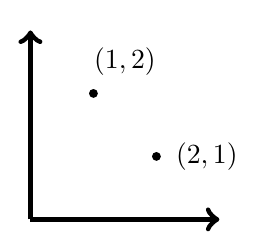
\begin{tikzpicture}[scale=0.8]
\draw[line width = 2pt,->] (0,0) -- (3,0);
\draw[line width = 2pt,->] (0,0) -- (0,3);
\fill (2,1) circle (2pt); \node at (2.8,1) {$(2,1)$};
\fill (1,2) circle (2pt); \node at (1.5,2.5) {$(1,2)$};
\end{tikzpicture}
\end{figure}\pause
\item A natural number, e.g. $172$ is $\{1,7,2\}$.\pause
\item An English word, e.g. \{C,h,e,e,r,s\}.\pause
\end{itemize}
\begin{block}{Equality of lists}
Two lists are \textbf{equal} provided they have the same length, and elements in the corresponding positions on the two lists are equal.
\end{block}
\center{E.g. lists $(a,b,c)$ and $(x,y,z)$ are equal if\\ $a=x$, $b=y$, and $c=z$.}
\end{frame}

\begin{frame}[t]{Counting two element lists}
\begin{block}{Question}
How many ordered pairs are there where the entries in the list may be any of the digits $1,2,3$, and $4$?
\end{block}\pause
Write out all possibilities:
\[
\begin{array}{cccc}
(1,1)&(1,2)&(1,3)&(1,4)\\
(2,1)&(2,2)&(2,3)&(2,4)\\
(3,1)&(3,2)&(3,3)&(3,4)\\
(4,1)&(4,2)&(4,3)&(4,4)
\end{array}
\]
\only<3>{We wrote this in a manner ensuring we have neither repeated nor omitted any such lists.}
\only<4>{
\begin{itemize}
\item First row contains all lists beginning with $1$, second row contains the ones beginning with $2$, etc.
\item There are $4$ such rows.
\item Each row contains four lists.
\end{itemize}}
\only<5>{\center{\alert{There are $16$ such lists.}}}
\end{frame}

\begin{frame}{Counting two element lists}
\begin{block}{Question}
How many ordered pairs are there where the entries in the list may be any of the digits $1,2,3,\dots,n$?
\end{block}\pause

\[
\begin{array}{cccc}
(1,1)&(1,2)&\dots&(1,n)\\
(2,1)&(2,2)&\dots&(2,n)\\
\vdots&\vdots&\ddots&\vdots\\
(n,1)&(n,2)&\dots&(n,n)
\end{array}
\]\pause
There are $n$ rows, each containing $n$ elements.\pause
\center{\alert{There are $n\cdot  n=n^2$ such lists.}}
\end{frame}

\begin{frame}{Counting two element lists}
\begin{block}{Question}
How many ordered pairs are there for which there are $n$ choices for the first element and $m$ choices for the second one?
\end{block}\pause

\[
\begin{array}{cccc}
(1,1)&(1,2)&\dots&(1,m)\\
(2,1)&(2,2)&\dots&(2,m)\\
\vdots&\vdots&\ddots&\vdots\\
(n,1)&(n,2)&\dots&(n,m)
\end{array}
\]\pause
There are $n$ rows, each containing $m$ elements.\pause
\center{\alert{There are $n\cdot m$ such lists.}}
\end{frame}

\begin{frame}{Counting two element lists}
\begin{block}{Question}
How many ordered pairs are there where the entries in the list may be any of the digits $1,2,3,4,5$, but where the two numbers in the list are different?
\end{block}\pause
\[
\begin{array}{ccccc}
-&(1,2)&(1,3)&(1,4)&(1,5)\\
(2,1)&-&(2,3)&(2,4)&(2,5)\\
(3,1)&(3,2)&-&(3,4)&(3,5)\\
(4,1)&(4,2)&(4,3)&-&(4,5)\\
(5,1)&(5,2)&(5,3)&(5,4)& -
\end{array}
\]\pause
\begin{itemize}
\item There are $5$ rows, each containing $4$ elements. \pause
\item $5$ choices for the first element and $4$ for the second. \pause
\item The choices are not independent, but that doesn't matter.
\end{itemize}\pause
\center{\alert{There are $5\cdot 4=20$ such lists.}}
\end{frame}

\begin{frame}
\begin{block}{Theorem (Multiplication Principle)}
Consider two-element lists for which there are $n$ choices for the first element, and for each choice of the first element, there are $m$ choices for the second element. Then the number of such lists is $nm$.
\end{block}\pause

\begin{proof}
Construct a chart of all possible lists. Each row of this chart contains all the two-element lists that begin with a particular element. Since there are $n$ choices for the first element, there are $n$ rows in the chart. Since, for each choice of the first element, there are $m$ choices for the second element, we know that every row of the chart has $m$ entries. Therefore the number of lists is
\[
\underbrace{m+m+\dots+m}_{n~times} = n\times m
\]
\end{proof}
\end{frame}

\begin{frame}[t]{Longer lists}
\begin{block}{Question}
How many lists of length three are there where the entries in the list may be any of the digits $1,2,3$?
\end{block}
\only<2>{
\[
\begin{array}{ccc}
(1,1,1)&(1,1,2)&(1,1,3)\\
(1,2,1)&(1,2,2)&(1,2,3)\\
(1,3,1)&(1,3,2)&(1,3,3)\\
(2,1,1)&(2,1,2)&(2,1,3)\\
(2,2,1)&(2,2,2)&(2,2,3)\\
(2,3,1)&(2,3,2)&(2,3,3)\\
(3,1,1)&(3,1,2)&(3,1,3)\\
(3,2,1)&(3,2,2)&(3,2,3)\\
(3,3,1)&(3,3,2)&(3,3,3)\\
\end{array}
\]}
\only<3->{
\[
\begin{array}{ccc}
(1,1,1)&(1,1,2)&(1,1,3)\\
(1,2,1)&(1,2,2)&(1,2,3)\\
\vdots&\vdots&\vdots\\
(3,2,1)&(3,2,2)&(3,2,3)\\
(3,3,1)&(3,3,2)&(3,3,3)\\
\end{array}
\]}
\only<4>{
\begin{itemize}
\item Every row of the chart corresponds to a fixed combination of the first two elements.
\item Every row consists of $3$ elements.
\item How many rows are there in this chart?
\end{itemize}}
\only<5>{
\begin{itemize}
\item How many rows are there in this chart?
\end{itemize}
We have solved this problem!$\qquad\to\qquad$ $3\times 3=9$.}
\only<6>{
\begin{itemize}
\item How many rows are there in this chart?$\quad\to$ $3\times 3=9$
\end{itemize}
\center{\alert{There are $9\times 3=3\times 3\times 3=27$ such lists.}}
}
\end{frame}

\begin{frame}

\begin{block}{Question}
How many lists of length three are there where the entries in the list may be any of the digits $1,2,3,4,5$ in which no number is repeated?
\end{block}\pause

We could write out the chart again but rather think:
\begin{itemize}
\item For the first element, we have $5$ choices.\pause
\item For the second element, we have to choose from the $4$ remaining.\pause
\item For the third place, we have to choose from the $3$ remaining.
\end{itemize}\pause

\center{\alert{There are $5\times 4\times 3=60$ such lists.}}

\end{frame}

\begin{frame}{In general}
How many lists are there of length $k$, in which each element of the list is selected from among $n$ possibilities.
\begin{enumerate}
\item Repetitions allowed:
\begin{block}{}
\[
\underbrace{n\times n\times\dots\times n}_{k~times}=n^k
\]
\end{block}
\item Repetitions not allowed: 
\begin{block}{}
\[
n\times(n-1)\times(n-2)\times\dots\times n-(k-1)
\]
\uncover<3>{when $k\leq n$, and $0$ if $k>n$.}
\end{block}
\uncover<2->{Is the second formula okay? What about $n=2$, $k=4$?}

\end{enumerate}

\end{frame}

\begin{frame}{In general}
\begin{block}{Notation}
The number
\[
(n)_k=n(n-1)(n-2)\dots (n-k+1)
\]
is called \textbf{falling factorial}.
\end{block}\pause

\begin{theorem}
The number of lists of length $k$ whose elements are chosen from a pool of $n$ possible elements is
\[
=\left\{\begin{array}{cc}
n^k&\textrm{if repetitions are permitted}\\
(n)_k&\textrm{if repetitions are forbidden}
\end{array}\right.
\]
\end{theorem}
\end{frame}


\end{document}